%!TEX program = xelatex
\documentclass[11pt]{beamer}

\usepackage{amsfonts}
\usepackage{amsmath}
\usepackage{blindtext}
\usepackage{enumitem}

\usetheme{SaoPaulo}

\title{Python Basics!}
\subtitle{data types, strings, indexing}
\author{CS101 Lecture \#3}
\date{2016-08-29}

\setcounter{showSlideNumbers}{1}

\begin{document}
  \setcounter{showProgressBar}{0}
  \setcounter{showSlideNumbers}{0}

%%%%%%%%%%%%%%%%%%%%%%%%%%%%%%%%%%%%%%%%%%%%%%%%%%%%%%%%%%%%%%%%%%%%%%%%%%%%%%%%
\frame{\titlepage}

%%%%%%%%%%%%%%%%%%%%%%%%%%%%%%%%%%%%%%%%%%%%%%%%%%%%%%%%%%%%%%%%%%%%%%%%%%%%%%%%
\setcounter{framenumber}{0}
\setcounter{showProgressBar}{1}
\setcounter{showSlideNumbers}{1}

%%%%%%%%%%%%%%%%%%%%%%%%%%%%%%%%%%%%%%%%%%%%%%%%%%%%%%%%%%%%%%%%%%%%%%%%%%%%%%%%
\section{Administrivia}

%%%%%%%%%%%%%%%%%%%%%%%%%%%%%%%%%%%%%%%%%%%%%%%%%%%%%%%%%%%%%%%%%%%%%%%%%%%%%%%%
\begin{frame}
  \frametitle{Administrivia}
  \Enlarge
  \begin{itemize}
  \myitem  Register your i>clickers on the course Compass page.
  \myitem  Complete Homework \#1 before Wednesday at 5:00 p.m.
  %\myitem  Homework \#2 will be assigned on Tuesday, due Friday Sep.\ 9.
  \myitem  Lab \#2 this week, no lab next week (Labor Day).
  \end{itemize}
\end{frame}

%%%%%%%%%%%%%%%%%%%%%%%%%%%%%%%%%%%%%%%%%%%%%%%%%%%%%%%%%%%%%%%%%%%%%%%%%%%%%%%%
\section{Warmup Quiz}

%%%%%%%%%%%%%%%%%%%%%%%%%%%%%%%%%%%%%%%%%%%%%%%%%%%%%%%%%%%%%%%%%%%%%%%%%%%%%%%%
\begin{frame}
  \frametitle{Our execution model}
  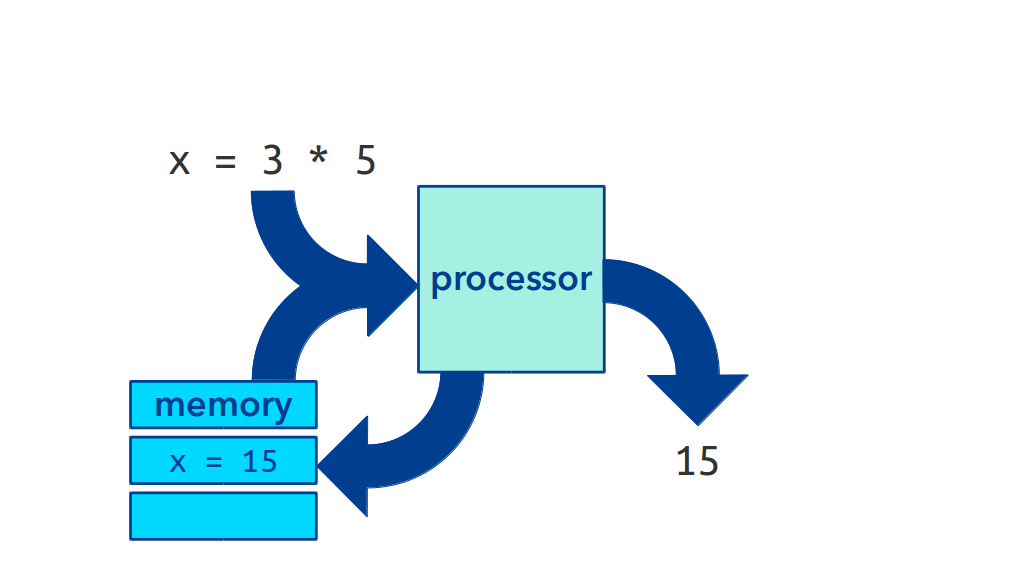
\includegraphics[width=\textwidth]{./img/computer-process.png}
\end{frame}

%%%%%%%%%%%%%%%%%%%%%%%%%%%%%%%%%%%%%%%%%%%%%%%%%%%%%%%%%%%%%%%%%%%%%%%%%%%%%%%%
\begin{frame}[fragile]
  \frametitle{Question \#1}
  \Enlarge

  \begin{semiverbatim}
x = 10
y = x + 1
y = x * y
  \end{semiverbatim}
  What is the value of \texttt{y}?
  \begin{enumerate}[label=\Alph*]
  \item  11
  \item  100
  \item  110
  \item  None of the above
  \end{enumerate}
\end{frame}

%%%%%%%%%%%%%%%%%%%%%%%%%%%%%%%%%%%%%%%%%%%%%%%%%%%%%%%%%%%%%%%%%%%%%%%%%%%%%%%%
\begin{frame}[fragile]
  \frametitle{Question \#2}
  \Enlarge

  \begin{semiverbatim}
x = 10
y = x + 1
y = x * y
  \end{semiverbatim}
  What do we call \texttt{x}?
  \begin{enumerate}[label=\Alph*]
  \item  a literal
  \item  a variable
  \item  an expression
  \item  a statement
  \end{enumerate}
\end{frame}

%%%%%%%%%%%%%%%%%%%%%%%%%%%%%%%%%%%%%%%%%%%%%%%%%%%%%%%%%%%%%%%%%%%%%%%%%%%%%%%%
\begin{frame}[fragile]
  \frametitle{Question \#3}
  \Enlarge

  \begin{semiverbatim}
x = 10
y = x + 1
y = x * y
  \end{semiverbatim}
  What do we call \texttt{10}?
  \begin{enumerate}[label=\Alph*]
  \item  a literal
  \item  a variable
  \item  an expression
  \item  a statement
  \end{enumerate}
\end{frame}

%%%%%%%%%%%%%%%%%%%%%%%%%%%%%%%%%%%%%%%%%%%%%%%%%%%%%%%%%%%%%%%%%%%%%%%%%%%%%%%%
\begin{frame}[fragile]
  \frametitle{Question \#2}
  \Enlarge

  \begin{semiverbatim}
x = 10
y = x + 1
y = x * y
  \end{semiverbatim}
  What do we call \texttt{y = x * y}?
  \begin{enumerate}[label=\Alph*]
  \item  a literal
  \item  a variable
  \item  an expression
  \item  a statement
  \end{enumerate}
\end{frame}

%%%%%%%%%%%%%%%%%%%%%%%%%%%%%%%%%%%%%%%%%%%%%%%%%%%%%%%%%%%%%%%%%%%%%%%%%%%%%%%%
\begin{frame}[fragile]
  \frametitle{Question \#5}
  \Enlarge

  \begin{semiverbatim}
x = 10
y = x
x = 5
  \end{semiverbatim}
  What is the value of \texttt{y}?
  \begin{enumerate}[label=\Alph*]
  \item  10
  \item  5
  \end{enumerate}
\end{frame}

%%%%%%%%%%%%%%%%%%%%%%%%%%%%%%%%%%%%%%%%%%%%%%%%%%%%%%%%%%%%%%%%%%%%%%%%%%%%%%%%
\section{Data Types}

%%%%%%%%%%%%%%%%%%%%%%%%%%%%%%%%%%%%%%%%%%%%%%%%%%%%%%%%%%%%%%%%%%%%%%%%%%%%%%%%
\begin{frame}
  \frametitle{What is an \textbf{encoding}?}
  \Enlarge

  \texttt{01001000 01000101 01001100 01001100} \\
  What does this binary data value represent?
  \begin{itemize}
  \myitem  What does this binary data represent? \pause
  \myitem  How does the processor know? \pause
  \myitem  The \textbf{encoding} interprets the value.
  \end{itemize}
\end{frame}

%%%%%%%%%%%%%%%%%%%%%%%%%%%%%%%%%%%%%%%%%%%%%%%%%%%%%%%%%%%%%%%%%%%%%%%%%%%%%%%%
\begin{frame}
  \frametitle{What is a \textbf{data type}?}
  \Enlarge

  \begin{itemize}
  \myitem  A \textbf{data type} defines an encoding rule.
  \myitem  All values have a type. \pause
  \myitem  The type defines how data is represented in memory. \pause
  \myitem  The type defines allowed operations and how they work.
  \end{itemize}
\end{frame}

%%%%%%%%%%%%%%%%%%%%%%%%%%%%%%%%%%%%%%%%%%%%%%%%%%%%%%%%%%%%%%%%%%%%%%%%%%%%%%%%
\begin{frame}
  \frametitle{Example}
  \Enlarge

  \texttt{01100111} can be the number \texttt{103}, the letter \texttt{g}, hexadecimal \texttt{67}, \texttt{3.5}, etc.
  \begin{itemize}
  \myitem  So what are these data types?
  \end{itemize}
\end{frame}

%%%%%%%%%%%%%%%%%%%%%%%%%%%%%%%%%%%%%%%%%%%%%%%%%%%%%%%%%%%%%%%%%%%%%%%%%%%%%%%%
\section{Numeric Data Types}

%%%%%%%%%%%%%%%%%%%%%%%%%%%%%%%%%%%%%%%%%%%%%%%%%%%%%%%%%%%%%%%%%%%%%%%%%%%%%%%%
\begin{frame}
  \frametitle{How do binary numbers work?}
  \Enlarge

  \begin{itemize}
  \myitem  Numeric types can be represented in binary:
    \begin{tabular}{*{27}{l}}
      \texttt{000} & 0 & \texttt{100} & 4 \\
      \texttt{001} & 1 & \texttt{101} & 5 \\
      \texttt{010} & 2 & \texttt{110} & 6 \\
      \texttt{011} & 3 & \texttt{111} & 7 \\
    \end{tabular} \pause
  \myitem  If we add more, the number \textbf{overflows}. \pause
  \myitem  Negative numbers?  Add a \textbf{sign bit}.
  \end{itemize}
\end{frame}

%%%%%%%%%%%%%%%%%%%%%%%%%%%%%%%%%%%%%%%%%%%%%%%%%%%%%%%%%%%%%%%%%%%%%%%%%%%%%%%%
\begin{frame}
  \frametitle{Integers, $\mathbb{Z}$}
  \Enlarge

  \begin{itemize}
  \myitem  Integers have been our only type thus far. \\
    $$ ..., -4, -3, -2, -1, 0, +1, +2, +3, ... $$
  \myitem  What are limits?
  \end{itemize}
\end{frame}

%%%%%%%%%%%%%%%%%%%%%%%%%%%%%%%%%%%%%%%%%%%%%%%%%%%%%%%%%%%%%%%%%%%%%%%%%%%%%%%%
\begin{frame}
  \frametitle{Integer operations}
  \Enlarge

  \begin{itemize}
  \myitem  Evaluating an expression of integers will generally result in an integer answer
    \begin{itemize}
    \mysubitem  \texttt{3 + 5}
    \mysubitem  \textcolor{red}{EXCEPTION:  DIVISION!} \pause
    \mysubitem  \texttt{3 / 4 $\rightarrow$ 0.75}
    \mysubitem  \texttt{3 // 4 $\rightarrow$ 0} (floor division)
    \end{itemize}
  \end{itemize}
\end{frame}

%%%%%%%%%%%%%%%%%%%%%%%%%%%%%%%%%%%%%%%%%%%%%%%%%%%%%%%%%%%%%%%%%%%%%%%%%%%%%%%%
\begin{frame}
  \frametitle{Floating-point numbers, $\mathbb{R}$}
  \Enlarge

  \begin{itemize}
  \myitem  Floating-point numbers include a fractional part. \\
    \textcolor{CS101GradBot}{(Anything with a decimal point---\texttt{2.4}, \texttt{3.0}.)} \pause
  \myitem  What are limits? \pause
    \begin{itemize}
    \mysubitem  Overflow/underflow
    \mysubitem  Arbitrary precision ($\pi$, $\mathbb{e}$)
    \end{itemize}
  \end{itemize}
\end{frame}

%%%%%%%%%%%%%%%%%%%%%%%%%%%%%%%%%%%%%%%%%%%%%%%%%%%%%%%%%%%%%%%%%%%%%%%%%%%%%%%%
\begin{frame}
  \frametitle{Floating-point operations}
  \Enlarge

  \begin{itemize}
  \myitem  Evaluating an expression of floating-point values will result in a floating-point answer. \pause
    \begin{itemize}
    \mysubitem  \texttt{3.0 + 5.5 $\rightarrow$ 8.5}
    \mysubitem  \texttt{3.0 + 5.0 $\rightarrow$ 8.0}
    \mysubitem  \texttt{3   + 5.5 $\rightarrow$ ?} (what happens here?)
    \end{itemize} \pause
  \myitem  Engineers and scientists need to think carefully about the precision of answers.
  \end{itemize}
\end{frame}

%%%%%%%%%%%%%%%%%%%%%%%%%%%%%%%%%%%%%%%%%%%%%%%%%%%%%%%%%%%%%%%%%%%%%%%%%%%%%%%%
\begin{frame}
  \frametitle{Complex numbers, $\mathbb{C}$}
  \Enlarge

  \begin{itemize}
  \myitem  Represent numbers with an imaginary component. \pause
  \myitem  Use \texttt{j} for $i$: \\
    \textcolor{CS101GradBot}{\texttt{1.0 + 1j}} \pause
  \myitem  Think of "jmaginary" numbers, I suppose.
  \end{itemize}
\end{frame}

%%%%%%%%%%%%%%%%%%%%%%%%%%%%%%%%%%%%%%%%%%%%%%%%%%%%%%%%%%%%%%%%%%%%%%%%%%%%%%%%
\begin{frame}[fragile]
  \frametitle{Example}
  \Enlarge

  \begin{semiverbatim}
x = 4
y = 3 + 1j
z = 33.3333
print( x + y + z )
  \end{semiverbatim}
  What is printed to the screen?
  \begin{enumerate}[label=\Alph*]
  \item  \texttt{40}
  \item  \texttt{40.3333}
  \item  \texttt{40.3333 + 1j}
  \item  None of the above
  \end{enumerate}
\end{frame}

%%%%%%%%%%%%%%%%%%%%%%%%%%%%%%%%%%%%%%%%%%%%%%%%%%%%%%%%%%%%%%%%%%%%%%%%%%%%%%%%
\begin{frame}
  \frametitle{Attribute operator \textbf{.}}
  \Enlarge

  \begin{itemize}
  \myitem  Reaches inside of a value to access part of its data (called an attribute). \pause
  \myitem  Extracts special variables stored “inside” the type.
    \begin{semiverbatim}
print(x.real)
print(x.imag)
    \end{semiverbatim} \pause
  \myitem  Both of these components are floats.
  \end{itemize}
\end{frame}

%%%%%%%%%%%%%%%%%%%%%%%%%%%%%%%%%%%%%%%%%%%%%%%%%%%%%%%%%%%%%%%%%%%%%%%%%%%%%%%%
\begin{frame}[fragile]
  \frametitle{Example}
  \Enlarge

  \begin{semiverbatim}
x = (3.5 + 1j)
y = 1
z = x + y
  \end{semiverbatim}
  What is the value of \texttt{z.imag}?
  \begin{enumerate}[label=\Alph*]
  \item  \texttt{4.5 + 1j}
  \item  \texttt{4.5}
  \item  \texttt{1j}
  \item  \texttt{1.0}
  \end{enumerate}
\end{frame}

%%%%%%%%%%%%%%%%%%%%%%%%%%%%%%%%%%%%%%%%%%%%%%%%%%%%%%%%%%%%%%%%%%%%%%%%%%%%%%%%
\section{String Data Type}

%%%%%%%%%%%%%%%%%%%%%%%%%%%%%%%%%%%%%%%%%%%%%%%%%%%%%%%%%%%%%%%%%%%%%%%%%%%%%%%%
\begin{frame}
  \frametitle{How does text work?}
  \Enlarge

  \begin{itemize}
  \myitem  Each symbol is stored individually, one byte long:
    \begin{tabular}{*{27}{l}}
      \texttt{01001000} & 72 \\
      \texttt{01000101} & 69 \\
      \texttt{01001100} & 76 \\
      \texttt{01001100} & 76 \\
      \texttt{01001111} & 79 \\
    \end{tabular}
  \end{itemize}
\end{frame}

%%%%%%%%%%%%%%%%%%%%%%%%%%%%%%%%%%%%%%%%%%%%%%%%%%%%%%%%%%%%%%%%%%%%%%%%%%%%%%%%
\begin{frame}
  \frametitle{ASCII encoding table}
  \Enlarge
  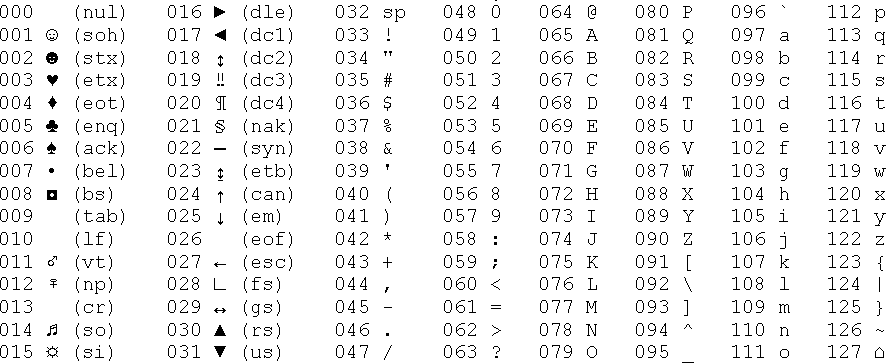
\includegraphics[width=\textwidth]{./img/ascii-table.png}
\end{frame}

%%%%%%%%%%%%%%%%%%%%%%%%%%%%%%%%%%%%%%%%%%%%%%%%%%%%%%%%%%%%%%%%%%%%%%%%%%%%%%%%
\begin{frame}
  \frametitle{ASCII encoding table}
  \Enlarge
  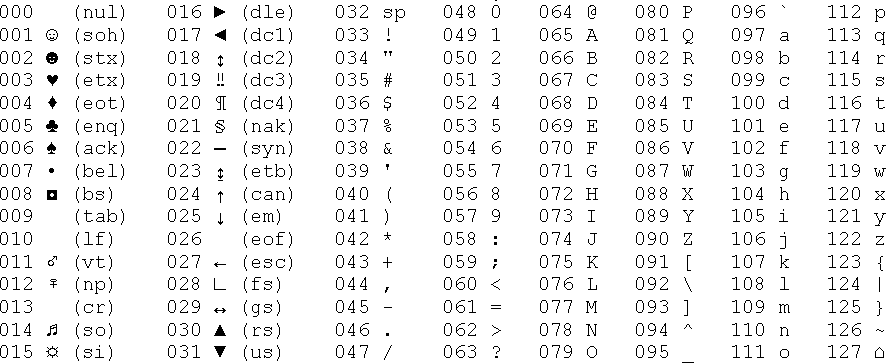
\includegraphics[width=\textwidth]{./img/ascii-table.png}

  \texttt{72 69 76 76 79} = ?
\end{frame}

%%%%%%%%%%%%%%%%%%%%%%%%%%%%%%%%%%%%%%%%%%%%%%%%%%%%%%%%%%%%%%%%%%%%%%%%%%%%%%%%
\begin{frame}
  \frametitle{ASCII encoding table}
  \Enlarge
  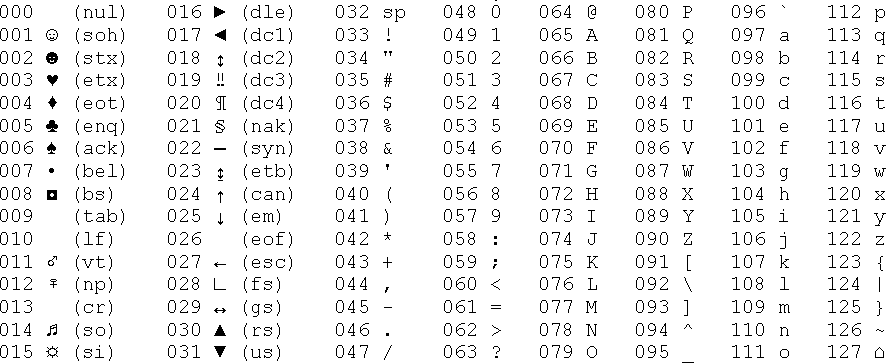
\includegraphics[width=\textwidth]{./img/ascii-table.png}

  \texttt{72 69 76 76 79} = \texttt{H E L L O}
  \texttt{'HELLO'}
\end{frame}

%%%%%%%%%%%%%%%%%%%%%%%%%%%%%%%%%%%%%%%%%%%%%%%%%%%%%%%%%%%%%%%%%%%%%%%%%%%%%%%%
\begin{frame}
  \frametitle{Strings}
  \Enlarge

  \begin{itemize}
  \myitem  As a literal:  text surrounded by quotes.
    \begin{itemize}
    \mysubitem  \texttt{"DEEP"}
    \end{itemize} \pause
  \myitem  Each symbol is a character. \pause
  \myitem  Unlike numeric types, strings vary in length.
  \end{itemize}
\end{frame}

%%%%%%%%%%%%%%%%%%%%%%%%%%%%%%%%%%%%%%%%%%%%%%%%%%%%%%%%%%%%%%%%%%%%%%%%%%%%%%%%
\begin{frame}
  \frametitle{String operations}
  \Enlarge

  \begin{itemize}
  \myitem  \textbf{Concatenation}:  combine two strings
    \begin{itemize}
    \mysubitem  Uses the \texttt{+} symbol
    \mysubitem  \texttt{'RACE' + 'CAR'}
    \end{itemize} \pause
  \myitem  \textbf{Repetition}:  repeat a string
    \begin{itemize}
    \mysubitem  Uses the \texttt{*}
    \mysubitem  \texttt{'HELLO '*10}
    \end{itemize} \pause
  \myitem  \textbf{Formatting}:  used to encode other data as string
    \begin{itemize}
    \mysubitem  Uses \texttt{\%} symbol
    \end{itemize}
  \end{itemize}
\end{frame}

%%%%%%%%%%%%%%%%%%%%%%%%%%%%%%%%%%%%%%%%%%%%%%%%%%%%%%%%%%%%%%%%%%%%%%%%%%%%%%%%
\begin{frame}[fragile]
  \frametitle{Formatting operator}
  \Enlarge

  \begin{itemize}
  \myitem  Creates string with value inserted \pause
    \begin{itemize}
    \mysubitem  Formats nicely
    \mysubitem  Requires indicator of type inside of string
    \end{itemize} \pause
  \begin{semiverbatim}
x = 100 * 54
s = "String is: %i" % x
print(s)
  \end{semiverbatim}
  \end{itemize}
\end{frame}

%%%%%%%%%%%%%%%%%%%%%%%%%%%%%%%%%%%%%%%%%%%%%%%%%%%%%%%%%%%%%%%%%%%%%%%%%%%%%%%%
\begin{frame}[fragile]
  \frametitle{Example}
  \Enlarge

  \begin{semiverbatim}
name = "Neal"
grade = 2 / 3
m1 = "Hello, %s!"" % name
m2 = "Your grade is:  %f" % grade
print(m1)
print(m2)
  \end{semiverbatim}
\end{frame}

%%%%%%%%%%%%%%%%%%%%%%%%%%%%%%%%%%%%%%%%%%%%%%%%%%%%%%%%%%%%%%%%%%%%%%%%%%%%%%%%
\begin{frame}[fragile]
  \frametitle{Example}
  \Enlarge

  \begin{semiverbatim}
x = 3
s = ("%i" % (x+1)) * x**(5%x)
print(s)
  \end{semiverbatim}

  What does this program print?
  \begin{enumerate}[label=\Alph*]
  \item  \texttt{333333333333}
  \item  \texttt{444444444}
  \item  \texttt{9999}
  \item  \texttt{\%i\%i\%i\%i\%i}
  \end{enumerate}
\end{frame}

%%%%%%%%%%%%%%%%%%%%%%%%%%%%%%%%%%%%%%%%%%%%%%%%%%%%%%%%%%%%%%%%%%%%%%%%%%%%%%%%
\begin{frame}[fragile]
  \frametitle{Indexing operator}
  \Enlarge

  \begin{itemize}
  \myitem  Extracts single character \pause
\begin{semiverbatim}
a = "FIRE"
a[0]
\end{semiverbatim} \pause
  \myitem  The integer is the index. \pause
  \myitem  \textcolor{red}{We count from zero!} \pause
  \myitem  If negative, counts down from end.
  \end{itemize}
\end{frame}

%%%%%%%%%%%%%%%%%%%%%%%%%%%%%%%%%%%%%%%%%%%%%%%%%%%%%%%%%%%%%%%%%%%%%%%%%%%%%%%%
\begin{frame}[fragile]
  \frametitle{Question}
  \Enlarge

  \begin{semiverbatim}
s = "ABCDE"
i = 3
x = s[i]
  \end{semiverbatim}

  What is the value of \texttt{x}?
  \begin{enumerate}[label=\Alph*]
  \item  \texttt{'A'}
  \item  \texttt{'B'}
  \item  \texttt{'C'}
  \item  \texttt{'D'}
  \item  \texttt{'E'}
  \end{enumerate}
\end{frame}

%%%%%%%%%%%%%%%%%%%%%%%%%%%%%%%%%%%%%%%%%%%%%%%%%%%%%%%%%%%%%%%%%%%%%%%%%%%%%%%%
\begin{frame}[fragile]
  \frametitle{Question}
  \Enlarge

  \begin{semiverbatim}
s = "ABCDE"
i = 25 % 3
y = s[i]
  \end{semiverbatim}

  What is the value of \texttt{y}?
  \begin{enumerate}[label=\Alph*]
  \item  \texttt{'A'}
  \item  \texttt{'B'}
  \item  \texttt{'C'}
  \item  \texttt{'D'}
  \item  \texttt{'E'}
  \end{enumerate}
\end{frame}

%%%%%%%%%%%%%%%%%%%%%%%%%%%%%%%%%%%%%%%%%%%%%%%%%%%%%%%%%%%%%%%%%%%%%%%%%%%%%%%%
\begin{frame}[fragile]
  \frametitle{Question}
  \Enlarge

  \begin{semiverbatim}
s = "ABCDE"
i = (11 % 3) - 7
z = s[i]
  \end{semiverbatim}

  What is the value of \texttt{z}?
  \begin{enumerate}[label=\Alph*]
  \item  \texttt{'A'}
  \item  \texttt{'B'}
  \item  \texttt{'C'}
  \item  \texttt{'D'}
  \item  \texttt{'E'}
  \end{enumerate}
\end{frame}

%%%%%%%%%%%%%%%%%%%%%%%%%%%%%%%%%%%%%%%%%%%%%%%%%%%%%%%%%%%%%%%%%%%%%%%%%%%%%%%%
\section{Reminders}

%%%%%%%%%%%%%%%%%%%%%%%%%%%%%%%%%%%%%%%%%%%%%%%%%%%%%%%%%%%%%%%%%%%%%%%%%%%%%%%%
\begin{frame}
  \frametitle{Reminders}
  \Enlarge

  \begin{itemize}
  \myitem  Register your i>clicker on Compass. \\ \textcolor{CS101GradBot}{(last chance before it counts!)}
  \myitem  Homework \#1 due Wednesday, Aug.\ 31, 5:00 p.m.
  \end{itemize}
\end{frame}

\end{document}
